\documentclass[a4paper,10pt,oneside,final,titlepage,onecolumn]{scrartcl}

\usepackage{ucs}
\usepackage[portuguese]{babel}
\usepackage[utf8x]{inputenc}
\usepackage[T1]{fontenc}
\usepackage{textcomp}
\usepackage{graphicx}
\usepackage{placeins}

\usepackage{listings}
\usepackage{color}

\definecolor{dkgreen}{rgb}{0,0.6,0}
\definecolor{gray}{rgb}{0.5,0.5,0.5}
\definecolor{mauve}{rgb}{0.58,0,0.82}

\setkomafont{disposition}{\normalfont\bfseries}

\lstset{frame=tb,
  language=bash,
  aboveskip=3mm,
  belowskip=3mm,
  showstringspaces=false,
  columns=flexible,
  basicstyle={\scriptsize\ttfamily},
  numbers=none,  
  breaklines=true,
  breakatwhitespace=true
  tabsize=3
}



\title{Trabalho 1 de MC833 --- Programação em Redes de Computadores}
\subtitle{Servidor de informação baseado em localização com socket TCP e UDP}
\author{Pedro Henrique Moura Andere, 105542, turma A\and Raul Rabelo Carvalho, 105607, turma A}



\begin{document}



\maketitle



\section{Introdução}
\paragraph{}O objetivo deste Trabalho foi a implementação em linguagem C de um sistema cliente/servidor para troca de informações sobre estabelecimentos comerciais em uma região e a comparação do desempenho deste sistema quando é empregado o protocolo TCP e quando o protocolo UDP é utilizado. Além disso, este Trabalho também compara a facilidade de implementação deste sistema nestes dois protocolos do ponto de vista do programador.
\paragraph{}Nas seções seguintes são descritos os métodos de armazenamento das informações, são mostrados os principais casos de uso do sistema e as decisões da implementação dos servidores e clientes são explicadas. Nas últimas seções, é feita a comparação entre o sistema usando TCP e o mesmo sistema usando UDP tanto quantitativamente, no caso do desempenho, quanto qualitativamente, em relação à facilidade na implementação do sistema.



\FloatBarrier

\section{Casos de uso do sistema}
\paragraph{}O sistema neste Trabalho utiliza um modelo de cliente/servidor, no qual existe um servidor de informação que acessa e processa os dados dos estabelecimentos cadastrados e um conjunto de clientes que requerem parte ou a totalidade dos dados para serem exibidos aos usuários.
\paragraph{}O sistema aceita comandos do usuário pelo \emph{software} cliente. Os comandos são:
\begin{description}
 \item[posicao <x>,<y>] --- informa a posição do usuário ao servidor.
 \item[posicao <x> <y>] --- idem o comando anterior.
 \item[categorias] --- exibe uma lista com os nomes das categorias de estabelecimentos existentes no sistema.
 \item[listar todos] --- exibe uma lista com o identificador (\emph{ID}) e nome de todos os estabelecimentos.
 \item[buscar todos] --- idem o comando anterior.
 \item[listar perto todos] --- exibe uma lista com o \emph{ID} e o nome dos estabelecimentos a menos de 100m da posição atual do usuário.
 \item[buscar perto todos] --- idem o comando anterior.
 \item[listar perto categoria <categoria>] --- exibe uma lista com o \emph{ID} e o nome dos estabelecimento a menos de 100 metros da posição atual do usuário e que sejam da categoria \verb|<categoria>|.
 \item[listar perto categoria <categoria>] --- idem o comando anterior.
 \item[listar categoria <categoria>] --- exibe uma lista com o \emph{ID} e o nome dos estabelecimentos da categoria \verb|<categoria>|.
 \item[buscar categoria <categoria>] --- idem o comando anterior.
 \item[info <ID>] --- exibe as informações do estabelecimento com \emph{ID} \verb|<ID>|.
 \item[votar <ID> <nota>] --- registra nas informações do estabelecimento com \emph{ID} \verb|<ID>| uma nota (inteiro \verb|<nota>| de 1 a 10) dada pelo usuário.
 \item[sair] --- encerra o cliente.
\end{description}

\subsection{Caso de uso: buscar por um estabelecimento próximo de uma categoria específica}
\begin{description}
 \item[Ator:] \hfill \\ Usuário do cliente.
 \item[Escopo:] \hfill \\ Sistema cliente/servidor.
 \item[Fluxo básico:] \hfill \\
 \begin{enumerate}
  \item Executar o cliente com os argumentos endereço IP e porta do servidor.
  \item Informar ao servidor a posição atual do cliente: \verb|posicao x,y|.
  \item Listar as categorias de estabelecimentos disponíveis: \verb|categorias|.
  \item Listar os estabelecimentos próximos da posição atual na categoria desejada: \verb|listar perto categoria <categoria>|.
  \item Exibir as informações do estabelecimento escolhido: \verb|info <ID>|.
  \item Encerrar o cliente: \verb|sair|.
 \end{enumerate}
 \item[Extenção:] \hfill \\ Após o passo 5, o usuário pode dar uma nota ao estabelecimento: \verb|votar <ID> <nota>|.
\end{description}

\subsection{Caso de uso: buscar por um estabelecimento próximo}
\begin{description}
 \item[Ator:] \hfill \\ Usuário do cliente.
 \item[Escopo:] \hfill \\ Sistema cliente/servidor.
 \item[Fluxo básico:] \hfill \\
 \begin{enumerate}
  \item Executar o cliente com os argumentos endereço IP e porta do servidor.
  \item Informar ao servidor a posição atual do cliente: \verb|posicao x,y|.
  \item Listar os estabelecimentos próximos da posição atual: \verb|listar perto todos|.
  \item Exibir as informações do estabelecimento escolhido: \verb|info <ID>|.
  \item Encerrar o cliente: \verb|sair|.
 \end{enumerate}
 \item[Extenção:] \hfill \\ Após o passo 4, o usuário pode dar uma nota ao estabelecimento: \verb|votar <ID> <nota>|.
\end{description}

\subsection{Caso de uso: buscar por um estabelecimento de uma categoria específica}
\begin{description}
 \item[Ator:] \hfill \\ Usuário do cliente.
 \item[Escopo:] \hfill \\ Sistema cliente/servidor.
 \item[Fluxo básico:] \hfill \\
 \begin{enumerate}
  \item Executar o cliente com os argumentos endereço IP e porta do servidor.
  \item Listar as categorias de estabelecimentos disponíveis: \verb|categorias|.
  \item Listar os estabelecimentos na categoria desejada: \verb|listar categoria <categoria>|.
  \item Exibir as informações do estabelecimento escolhido: \verb|info <ID>|.
  \item Encerrar o cliente: \verb|sair|.
 \end{enumerate}
 \item[Extenção:] \hfill \\ Após o passo 4, o usuário pode dar uma nota ao estabelecimento: \verb|votar <ID> <nota>|.
\end{description}

\subsection{Caso de uso: listar todos os estabelecimentos}
\begin{description}
 \item[Ator:] \hfill \\ Usuário do cliente.
 \item[Escopo:] \hfill \\ Sistema cliente/servidor.
 \item[Fluxo básico:] \hfill \\
 \begin{enumerate}
  \item Executar o cliente com os argumentos endereço IP e porta do servidor.
  \item Listar os todos os estabelecimentos cadastrados: \verb|listar todos|.
  \item Encerrar o cliente: \verb|sair|.
 \end{enumerate}
 \item[Extenção:] \hfill \\ Após o passo 2, o usuário pode:
 \begin{itemize}
  \item Exibir as informações de um estabelecimento: \verb|info <ID>|.
  \item Dar uma nota a um estabelecimento: \verb|votar <ID> <nota>|.
 \end{itemize}
\end{description}



\FloatBarrier

\section{Armazenamento e estruturas de dados}
\paragraph{}Cada estabelecimento cadastrado no servidor de informação foi modelado por uma estrutura de dados na linguagem C (\verb|struct item|) definida como um tipo \verb|item_t|. A estrutura contém cinco campos do tipo inteiro e três do tipo vetor de caracteres. Os campos são os seguintes:
\begin{description}
 \item[id] \hfill \\ (Inteiro.) O identificador único de cada estabelecimento.
 \item[posx] \hfill \\ (Inteiro.) A coordenada no eixo-x da posição do estabelecimento.
 \item[posy] \hfill \\ (Inteiro.) A coordenada no eixo-y da posição do estabelecimento.
 \item[categoria] \hfill \\ (Vetor de caracteres.) O nome da categoria ao qual o estabelecimento pertence.
 \item[nome] \hfill \\ (Vetor de caracteres.) O nome do estabelecimento.
 \item[endereco] \hfill \\ (Vetor de caracteres.) O endereço do estabelecimento.
 \item[pontuacao] \hfill \\ (Inteiro.) O total acumulado das notas dadas ao estabelecimento.
 \item[votos] \hfill \\ (Inteiro.) O total de vezes que o estabelecimento recebeu uma nota.
\end{description}
\paragraph{}Todos os inteiros são inteiros com sinal (apesar de que nenhum dos campos necessita armazenar valores negativos) e os vetores de caracteres têm todos comprimento máximo de 256 posições. Foi escolhido dar um tamanho máximo para esses campos, pois torna a implementação mais simples e menos propensa a erros; além disso, bancos de dados comumente trabalham com campos de tamanho fixo.
\paragraph{}Um vetor do tipo \verb|item_t| pode empregado para guardar na memória para uso pelo servidor uma parte ou a totalidade (como é o caso da implementação feita para este Trabalho) do conjunto de estabelecimentos cadastrados.
\paragraph{}Para o armazenamento permanente dos dados em disco, foi usado um arquivo de texto simples contendo por linha as informações de um estabelecimento, com cada campo separado por um ponto-e-vírgula. A ordem dos campos é a mesma da lista acima. A única exceção é a primeira linha que contém somente um inteiro com o número de estabelecimentos contidos no arquivo. É importante que esteve número esteja correto, pois o servidor irá ignorar qualquer entrada além da quantidade dada na primeira linha do arquivo, e irá encerrar com erro se o número de entradas for menor que esta quantidade.
\paragraph{}Outra estrutura de dados empregada pelo servidor é a estrutura do tipo \verb|res_busca_t| que contém dois campos: um inteiro para guardar identificadores e um vetor de caracteres (também com 256 posições) para armazenar nomes. Um vetor deste tipo é usado para passar o resultado de buscas sobre o conjunto de estabelecimentos para as funções de impressão e comunicação do servidor.



\FloatBarrier

\section{Detalhes da implementação}
\paragraph{}Os servidores de informação UDP e TCP utilizam ambos o mesmo conjunto de funções de manipulação de dados: leitura e escrita em disco e busca por dados específicos; enquanto as funções de comunicação por redes, ainda que similares, têm diferenças importantes devido ao modelo de comunicação (por conexão no TCP e por mensagens no UDP).
\paragraph{}A primeira decisão de implementação significativa é referente à escolha do armazemento permanente das informações em um arquivo de texto e da representação destas informações em memória volátil para uso nas buscas e consultas. O arquivo de texto é uma solução de escalabilidade limitada devido a ausência de estruturas de indexão como em um banco de dados. Conjuntos grandes de informação resultariam em perda de desempenho significativa durante consultas, pois o servidor precisaria quebrar as informações em subconjuntos. No entanto, como o interesse deste Trabalho é comparar o desempenho de servidores TCP contra servidores UDP, o conjunto de informações é pequeno o bastante para que o programa trabalhe com a totalidade dos dados, que são carregados no vetor \verb|listas| a cada busca ou consulta.
\paragraph{}Ambos os servidores foram projetados para ignorar comandos ilegais passados pelos clientes, somente retornando mensagens de erro ao cliente quando este emprega um dos comandos erroneamente, tal como é o caso de se tentar listar os estabelecimentos próximos antes de informar a posição do cliente.
\paragraph{}Como comunicação pelo protocolo UDP não mantém o estado de cada conexão com os clientes e, mais importante, não garante a entrega das mensagens enviadas, o servidor UDP procura mitigar os erros por omissão causados por perda de mensagens enviando uma mensagem de reconhecimento para cada mensagem recebida dos clientes. O cliente UDP espera pela mensagem de reconhecimento, mas não re-envia a mensagem original caso o reconhecimento não seja recebido; o cliente simplesmente avisa ao usuário que não houve resposta do servidor, deixando para o usuário que ele re-envie o comando. No sentido contrário, não há controle de recebimento das mensagens, ou seja, caso alguma mensagem do servidor seja perdida, o cliente não tem como identificar este tipo de erro. Nos dois casos, o não reconhecimento de um comando ou a resposta incompleta ou ausente, foi deixado para o usuário a identificação deste tipo de erro pois, caso fosse importante que a comunicação tivesse controle de falhas, o mais correto seria utilizar o protocolo TCP que já tem implementado essas ferramentas; e, no caso deste Trabalho, este sistema cliente/servidor TCP foram implementados e não necessitam nem mesmo do mecanismo simples de reconhecimento de comandos.
\paragraph{}Outro detalhe é por se poder utilizar a função \verb|connect| em um socket UCP, o que torna possível usar as mesmas funções para recembimento e envio de mensagens que são usadas com sockets TCP, o cliente UDP foi implementado estabelecendo uma ``conexão'' pelo socket UDP, o que simplificou a implementação do cliente UDP que pode ser bastante semelhante à versão TCP. 
\paragraph{}O servidor TCP é implementado para ser um servidor concorrente que cria processos-filhos para cada conexão com clientes estabelecida. Um detalhe importante no servidor TCP é que o comando \verb|sair| do cliente é enviado ao servidor, para que este possa encerrar o processo-filho corretamente. Isto é feito utilizando a biblioteca \verb|signal.h|, que configura um \emph{handler} para executar uma chamada de sistema que mata o processo sempre que este entrar no estado de espera.
\paragraph{}Finalmente, ambos os clientes, TCP e UDP, utilizam multiplexação de entrada e saída para poderem ``ouvir'' duas \emph{streams} diferentes: o socket de comunicação e a entrada padrão. No caso do cliente UDP, a função de multiplexação \verb|select| também foi usada como um \emph{timer} enquanto o cliente espera pela mensagem de reconhecimento vinda do servidor.
\paragraph{}Os programas foram escritos em linguagem C (glibc versão 2.19-3) e compilados para os testes pelo gcc versão 4.8.2-8 no sistema operacional ArchLinux (kernel 3.14.1-1). Para a medição dos tempos de consultas foi usado a ferramenta timer (GNU time versão 1.7).



\FloatBarrier

\section{Tempo de consulta}
\paragraph{}Para medir a diferença no desempenho de cada tipo de servidor implementado, foram preparados quatro arquivos de entrada de comandos que fazem cinco, dez, vinte e quarenta repetições de uma consulta seguindo um dos casos de uso do sistema. A consulta consiste dos comandos:
\begin{itemize}
 \item  posicao 100 100
 \item categorias
 \item listar perto categoria cafe
 \item info 1
\end{itemize}
\paragraph{}Após as repetições, o comando sair é enviado. O tempo de cada consulta foi medido com a ferramenta \verb|time|, executada da seguinte maneira:
\\ \verb|time cliente_info_TCP 10.17.23.103 23 < test05.bat|;
\\ a mesma linha de comando foi usada para o servidor UDP e o arquivo de entrada variou (test10.bat, test20.bat e test40.bat, além do mostrado na linha de comando). Cada teste foi repetido cinco vezes e foi tomada uma média para construir o gráfico abaixo.
\begin{figure}[!ht]
  \caption{Tempos de consulta.}
  \centering
  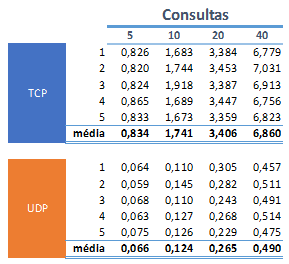
\includegraphics[width=70mm]{table-lan.png}
  \label{netstat}
\end{figure}
\begin{figure}[!ht]
  \caption{Gráfico do tempo médio de consulta.}
  \centering
  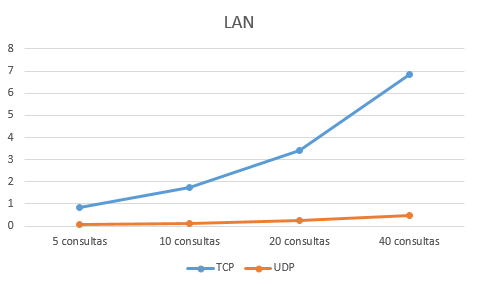
\includegraphics[width=117mm]{graph_lan.png}
  \label{netstat}
\end{figure}



\FloatBarrier

\section{Comparação}
\paragraph{}O tempo para uma consulta do tipo mostrado na seção anterior é para TCP de 0,151 s, em média, e para UDP é 0,010, também em média. Devido ao \emph{overhead} do estabelecimento da conexão e do controle de falhas e sequenciamento das mensagens no protocolo TCP, o tempo de cada consulta é muito superior ao tempo de consulta quando usando o servidor UDP. A ferramenta time mostra que o servidor TCP gasta a maior parte to tempo de execução em modo de sistema, que o tempo necessário para o \emph{kernel} Linux estabelecer a conexão, enviar as mensagens e verificar a presença de erros, já que as funções de leitura e escrita em disco são iguais em ambas as versões.
\paragraph{}O protocolo TCP se mostra ainda mais lento a medida em que se aumenta o número de consultas por conexão que são feitas. Enquanto o tempo médio do conjunto de consultas ao servidor UDP teve um crescimento aproximadamente linear a medida em que se dobrava o número de consultas, o tempo médio no caso do servidor TCP mostra uma curva de crescimento exponencial. Este resultado mostra que para aplicações em que o tempo de envio de mensagens é crítico, a implementação UDP tem uma escalabilidade muito mais atraente, sendo que para fluxos de mensagens muito intenso a solução em protocolo TCP torna-se inviável.
\paragraph{}Por outro lado, aplicações UDP requerem um maior cuidado caso se deseje algum tipo de controle de falhas. A implementação deste controle na aplicação pode resultar em ganho de desempenho mesmo mantendo-se uma robustez comparável a implementação em TCP, mas isso resulta em um código maior. No caso deste Trabalho, o único controle de falhas implementado foi um mecanismo de reconhecimento de comandos e mesmo assim o código teve um crescimento. No caso do servidor, foram 22081 caracteres na versão TCP e 21430 na versão UDP, um crescimento de 3\%. Mas no cliente, onde a maior parte do mecanismo de reconhecimento de comandos foi implementado, o cresimento foi de 24\%.
\paragraph{}No entanto, como o controle de erros do sistema cliente/servidor UDP é simples, a comfiabilidade nas respostas é baixa. É até mesmo difícil identificar se comando foi recebido mas a mensagem de reconhecimento se perdeu (junto com a mensagem com a resposta propriamente dita ao comando), ou se o servidor não está sendo executado. Como o protocolo UDP não garante a ordenação das mensagens, as respostas à consultas que são quebradas em várias mensagens podem ser recebidas fora de ordem. Um modo de se resolver este problema é o etiquetamento de cada mensagem com um número de sequência; outro mode seria o cliente conhecer o formato final da resposta de modo que ele possa identificar quais partes de uma resposta quebrada em várias mensagens não foi recebida. Mas para aplicações que podem conviver com um atraso na resposta maior, é mais conveniente usar os mecanismos de controle já existentes no protocolo TCP.
\paragraph{}Outro ponto em que a implementação de comunicação por redes empregando o protocolo TCP tem vantagens do ponto de vista do programador é o nível de abstração que existe nos sistemas Unix/Linux. Ao transpor todo o controle de ordenação e falhas para o sistema operacional e disponibilizar somente um socket ao qual uma conexão é estabelecida entre duas máquinas, o programador deixa de ter de se preocupar com erros por omissão de mensagens, recebimento de mensagens repetidas e reconhecimento de recebimento. O programador fica livre para se concentrar na lógica da aplicação.



\FloatBarrier

\section{Conclusão}
\paragraph{}Neste Trabalho foi mostrado que os dois protocolos de transporte mais empregados em redes de computadores exibem características que tornam cada um deles mais indicado para determinados tipos de aplicação. No caso do servidor de informações implementado, o protocolo TCP apresenta mais vantagens em relaçao ao protocolo UDP por ser este servidor pouco dependente de uma
resposta rápida como a implementação em UDP mostrou. As vantagens de facilidade de implementação e especialmente confiabilidade superam a vantagem da velocidade e escalabilidade do servidor UDP.
\paragraph{}No entanto, o resultado da medição do tempo para conjuntos grandes de consultas é importante, pois mostra claramente como o
\emph{overhead} do estabecimento da conexão TCP e os mecanismos de controle afetam o desempenho da aplicação: a aplicação usando TCP teve tempos de consulta aproximadamente um ordem de grandeza mais lento que a aplicação usando UDP e a diferenção aumentou com a medida em que se dobrava o conjunto de consultas.
\paragraph{}No geral, este Trabalho mostrou que os ganhos de desempenhos de uma aplicação usando UDP podem ser significativos, mas que o cuidado na implementação e o trabalho necessários para manter a mesma confiabilidade da mesma aplicação usando TCP podem não compensar os atrasos.

\end{document}
